\section{Uvod}
Algoritam krijesnica\cite{10.1007/978-3-642-04944-6_14} metaheuristički je optimizacijski algoritam sličan algoritmu rojeva čestica. Nadahnut je načinom na koji se krijesnice u prirodi međusobno privlače. 

Krijesnice imaju sposobnost međusobnog odašiljanja svjetlosnih signala svojim svjetlećim organima. Neke vrste odašilju trepteće, a neke konstanto svjetlo. Takvi signali služe za privlačenje partnera za parenje i privlačenje potencijalnog plijena. U nekim vrstama mužjaci privlače ženke, a u drugima obratno.


\section{Algoritam}
U samom algoritmu razmatramo međusobno privlačenje krijesnica. Potrebno je idealizirati svojstva svijetljenja:

\begin{enumerate}
	\item Ne razlikujemo muške i ženske krijesnice, sve svijetle i sve se međusobno privlače.
	\item Privlačnost je proporcionalna intenzitetu svjetla kojeg odašilju i opada kvadratom udaljenosti $I \propto \frac{1}{r^2}$. Ona krijesnica s većim intenzitetom svjetla privlači onu s manjim.
	\item Intenzitet svjetla krijesnice određen je funkcijom cilja.
\end{enumerate}



\subsection{Privlačnost}
Za intenzitet svjetla same krijesnice moguće je u najjednostavnijem slučaju uzeti $I_0(\vec{x}) \propto f(\vec{x})$ (za maksimizacijske probleme) ili $I_0(\vec{x}) \propto -f(\vec{x})$ (za minimizacijske probleme). Ključno je pitanje kakav intenzitet svjetla vide druge krijesnice, to jest koliku imaju privlačnost $\beta$.

Intenzitet svjetla na udaljenosti $r$ je:

\begin{equation}
	I(r) = \frac{I_0}{r^2}
\end{equation}

Apsorpcija svjetla okoline $\gamma$ je:

\begin{equation}
	I(r) = I_0 e^{-\gamma r}
\end{equation}

Ova dva izraza mogu se kombinirati u Gaussovoj formi čime se izbjegava nedefinirana vrijednost intenziteta svjetla na udaljenosti $r = 0$:

\begin{equation}
	I(r) = I_0 e^{-\gamma r^2}
\end{equation}

Mogu se upotrijebiti i druge monotono padajuće funkcije:

\begin{equation}
	I(r) = \frac{I_0}{1 + \gamma r^2}
\end{equation}

Kako se definirao intenzitet svjetlosti, tako se može definirati privlačnost:

\begin{equation}
	\beta(r) = \beta_0 e^{-\gamma r^2}
\end{equation}

Privlačnost se može definirati i kao bilo koja monotono padajuća funkcija oblika:

\begin{equation}
	\beta(r) = \beta_0 e^{-\gamma r^m}
\end{equation}


Karakteristična udaljenost $\Gamma$ je udaljenost na kojoj privlačnost opada s $\beta_0$ na $\beta_0e^{-1}$. Ona iznosi $\Gamma = \gamma^{\frac{-1}{m}}$. Isto tako, na temelju karakteristične udaljenosti nekog problema, može se odrediti konstanta apsorpcije svjetla $\gamma = \frac{1}{\Gamma^m}$

\subsection{Kretanje}
Položaj krijesnice predstavlja $n$-dimenzionalni vektor:
\begin{equation}
	\vec{x} = (x_1, x_2, \dots, x_n)
\end{equation}
Položaj $i$-te od $N$ krijesnica:
\begin{equation}
	\vec{x}_i = (x_{i1}, x_{i2}, \dots, x_{in})
\end{equation}
Udaljenost između krijesnica računamo euklidskom udaljenošću:
\begin{equation}
	r_{ij} = ||\vec{x}_i - \vec{x}_j|| = \sqrt{\sum_{k = 1}^{n}(x_{ik} - x_{jk})^2}
\end{equation} 
Kretanje krijesnice $i$ prema krijesnici $j$ većeg intenziteta svjetla je:
\begin{equation}
	\vec{x}_i \leftarrow \vec{x}_i + \beta_0e^{-\gamma r_{ij}^m}(\vec{x}_j - \vec{x}_i) + \alpha rand(-1, 1)
\end{equation}

Drugi pribrojnik predstavlja pomak u smjeru privlačne krijesnice, a treći predstavlja slučajni pomak. 

Uobičajeno je uzeti da su parametri $m = 2$, $\beta_0 = 1$ i $\alpha \in [0, 1]$. To ostavlja parametar $\gamma$ čiji odabir najviše utječe na konvergenciju algoritma, uobičajeno ga je odrediti na temelju karakteristične udaljenosti $\Gamma$.

\subsection{Pseudokod}

\begin{algorithm}[H]
	\begin{algorithmic}[1]
		\Function{FA}{n, N, maxGen, $\gamma$}
		
		\State X = \Call{Inicijalizacija}{n, d}
		\While{gen < maxGen}
		\For{i = 1 to n}
		\For{j = 1 to n}
		\If{I(X[j]) > I(X[i])} 
		\State Pomakni krijesnicu X[i] prema krijesnici X[j]
		\State Ažuriraj intenzitet svjetla krijesnice X[i]
		\EndIf
		\EndFor
		\EndFor
		\State Ažuriraj najbolje rješenje x*
		\EndWhile
		\State \Return x*	
		\EndFunction
	\end{algorithmic}
	\caption{Algoritam krijesnica}
\end{algorithm}

\section{Programsko ostvarenje}
\subsection{Programsko ostvarenje MEALPY}
Algoritam krijesnica i mnogi drugi metaheuristički algoritmi programski su ostvareni u sklopu knjižnice programa otvorenog koda \href{https://mealpy.readthedocs.io/en/latest}{MEALPY} programskog jezika Python. Knjižnica se može preuzeti naredbom konzole:


\begin{framed}
	\begin{verbatim}
		> pip install mealpy
	\end{verbatim}
\end{framed}

Prethodno opisani problem funkcije \eqref{eq:fx} s $n = 30$ definira se u programu kao rječnik i pokreće se algoritam krijesnica s 1000 epoha, brojem krijesnica $N = 50$,  $\gamma = 0.1$,  $\beta_0 = 1$, $\alpha = 0.5$ i $m = 2$:
\begin{framed}
	\begin{verbatim}
		import numpy as np
		from mealpy import FloatVar, FFA
		
		n = 30
		
		def objective_function(solution):
		return -np.sum(solution**2)
		
		problem = {
			"obj_func": objective_function,
			"bounds": FloatVar(lb=(-10., )*n, ub=(10., )*n),
			"minmax": "max",
		}
		
		
		model = FFA.OriginalFFA(epoch=1000, pop_size=50, 
		gamma = 0.1, beta_base = 1, 
		alpha = 0.5, exponent = 2)
		
		g_best = model.solve(problem)
		
		print("Solution:", g_best.solution)
		print("Fitness:", g_best.target.fitness)
	\end{verbatim}
\end{framed}


\noindent Izlaz ovog primjera je:
\begin{framed}
	\begin{verbatim}
		Solution: [-1.77332972  2.96553989 ...  -3.77894221]
		Fitness: -146.04412518749243
	\end{verbatim}
\end{framed}

\subsection{Programsko ostvarenje MQL5}
Programsko ostvarenje A. Dika u jeziku MQL5 može se preuzeti i pokrenuti na način analogan onom opisanom u odjeljku \ref{sec:mql5majmun}.

Primjer pokretanja \eqref{eq:fx} s $n = 30$ s 1000 epoha, $N = 50$,  $\gamma = 0.1$,  $\beta_0 = 1$, $\alpha = 0.5$:

\begin{figure}[H]
	\centering
	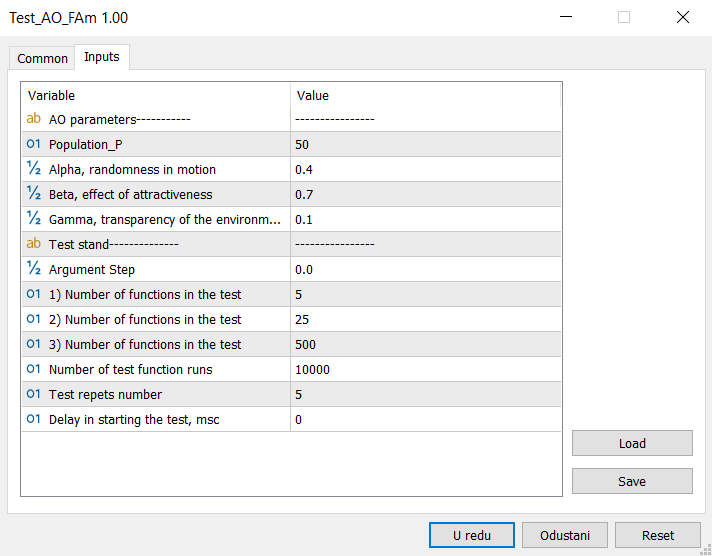
\includegraphics[width=14cm]{mt61}
	\caption{Odabir parametara algoritma za primjer}
	\centering
\end{figure}

\begin{figure}[H]
	\centering
	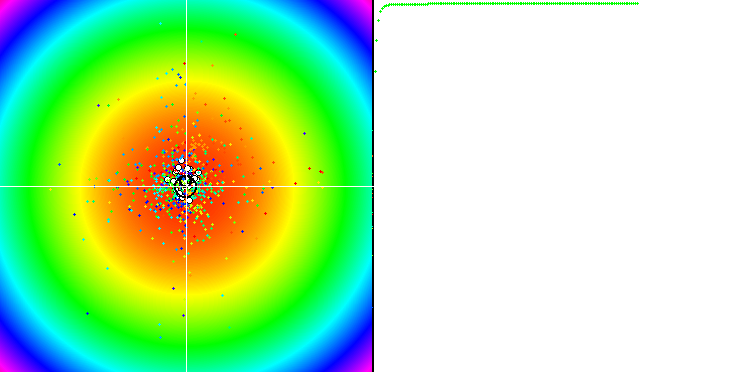
\includegraphics[width=14cm]{mt62}
	\caption{Položaji krijesnica na hiperravnini i izlazi funkcije cilja tijekom izvođenja}
	\centering
\end{figure}

\noindent Ispis je:
\begin{framed}
	\begin{verbatim}
		15 Sphere's; Func runs 10000 result: -70.09166510586255
		Score: 0.99650
	\end{verbatim}
\end{framed}



\section{Primjene}

\subsection{Economic Emissions Load Dispatch problem}
Algoritam krijesnica primijenjen je na problem \textit{Economic Emissions Load Dispatch} u kojem se istovremeno minimizira cijena i količina emisija stakleničkih plinova.\cite{Apostolopoulos2010} Pokazalo se da je uz pravilan odabir parametara moguće postići dobra rješenja.

\subsection{Kombinatorna optimizacija}
Hibridna inačica algoritma krijesnica, uz heuristiku lokalnog pretraživanja, upotrebljena je na problemu bojanja grafa s 3 boje.\cite{fister2012memetic} Rezultati su bili obećavajući i pokazali da je moguće koristiti algoritam i za druge kombinatorne probleme.


\subsection{Punjenje hladnjaka radi uštede energije}
Poboljšani algoritam krijesnica (IFA) korišten je za rješavanje problema punjenja hladnjaka.\cite{COELHO2013273} Imao je bolje performanse od nekoliko optimizacijskih algoritama iz literature.

\subsection{Segmentacija slika}
Algoritam krijesnica i algoritam $k$-NN korišteni su u kombinaciji za grupiranje piksela slika u $k$ grupa.\cite{7857598}

\subsection{Procjena potražnje vodenih resursa}
Novi dinamični algoritam krijesnica (NDFA) korišten je za procjenu potražnje vodenih resursa u gradu Nanchangu u Kini.\cite{WANG201895} Podaci o potražnji od 2003. do 2012. korišteni su za učenje modela, a predviđanje je ispitivano na podacima  od 2013. do 2015. Točnost predviđanja bila je $97.91\%$.

\subsection{Navigacija mobilnih robota u promjenjivim okolinama}
Navigacija grupe mobilnih robota u promjenjivim okolinama ostvarena je algoritmom krijesnica u kojem roboti predstavljaju krijesnice i vodeći se algoritmom, istražuju okolinu.\cite{PATLE2018691} Pokazalo se da su performanse ovog rješenja bolje nego drugih predloženih.

\subsection{Odabir značajki za detekciju upada na mrežma}
Algoritam krijesnica upotrebljen je za odabir značajki na temelju kojih se detektira upad.\cite{B2019148} Rezultat je pokazao je obećavajuć napredak u odnosu na druge prijedloge rješenja.

\subsection{Optimizacija životnog vijeka mreže bežičnih senzora}
Za optimizaciju životnog vijeka mreže bežičnih senzora korišten je poboljšani algoritam krijesnica (IFA).\cite{9148087} Simulacijama je pokazano da taj algoritam ima bolje i ujednačenije performanse od drugih algoritama.
